\documentclass[12pt,technote]{IEEEtran}
\usepackage{cite}
\usepackage{amsmath}
\usepackage{hyperref}
\usepackage{bookmark}
\usepackage{amssymb}
\usepackage{graphicx}
\usepackage{caption}
\usepackage{subcaption}
\usepackage{hyperref}
\usepackage{tikz}

\usetikzlibrary{shapes.geometric, arrows}

\hypersetup{
    colorlinks=true,
    linkcolor=blue,
    filecolor=magenta,
    urlcolor=cyan,
    pdfpagemode=FullScreen,
}

\author{Henry Pick, MATH189J}
\title{Algebraic Signal Processing Theory in Image Processing}
\date{3 April 2022}
\begin{document}
\maketitle
\begin{abstract}
    In this paper, we explore constructs in image processing through the work of Markus P\"uschel on algebraic signal processing theory. His main objective was to introduce well-established concepts in signal processing as a comprehensive algebraic theory. Here, we do much of the same, in fact a significant portion of this paper is devoted to reviewing essential ideas in his paper. We draw connections between abstract algebra and representation theory and the core concepts learned in many systems engineering classes. In my own effort to make this work original, I will explore several applied cases not covered in P\"uschel's work and design an image compression pipeline that makes use of several of P\"uschel's discussion points.
\end{abstract}
\section{Introduction}
In nearly all fields of the applied sciences, we interact with the broad definition of ``signal processing''. It is a term traditionally used in electrical engineering but has now found use in a wide range of other fields including image processing, wireless communication, financial analysis, and machine learning.

Signal processing deals with functions defined on sets, often times countable sets in the context of digital computing. We also have a set of functions, commonly referred to as ``filters'' that transform these signals. In this paper, we focus on linear signal processing, which means that this set of functions operates on signals \textit{linearly}. That is, given a transformation $A$, signals $x$ and $y$, and scalar multiples $r_1$ and $r_2$ it holds that $A(r_1x + r_2y) = r_1A(x) + r_2A(y)$, which is still a signal.

Some with experience in one of the fields of signal processing may find this last sentence fairly straightforward, drawing on some assumptions. If one had contextualized this as the processing of complex digital sensor data, they might have assumed that $x$ and $y$ live in the vector space $\mathbb{C}^n$ over the field $\mathbb{C}$ and that the expression $r_1x + r_2y$ is simply the vector sum of $x$ and $y$ scaled by $r_1$ and $r_2$. Reading this last sentence from an abstract algebra perspective should have seemed slightly awkward, however. Since we have not given an algebraic foundation for these objects $A, x, y, r_1,$ and $r_2$, we have no conception of how the interact with one another, how we might represent these objects linearly, and what a signal generally represents. The instinct of the mathematician is to establish a comprehensive theory that characterizes features common to all signal processing contexts. This is exactly what Markus P\"uschel has done in his work on algebraic signal processing theory\cite{AlgebraicSignalProcessing2006}.

One might question the practical value of an algebraic exploration of an already well-established science. In this inquiry, we find many justifications that apply far beyond the mathematics alone. For example, an engineer who has significant experience in one field of signal processing may find a natural means of recognizing parallels in an entirely different field. It also becomes clear that signal processing optimizations which are seemingly the product of ingenious creativity are actually quite procedural in their construction. The design of fast fourier transform algorithms, for example, can be as simple as observing the symmetry structure of an underlying signal module.

This paper will first explore the foundational concepts of algebraic signal processing, which is primarily an expository section. We also consider some ideas that were not addressed in this work and potential extensions for P\"uschel's signal processing theory. We then move on to a practical application of constructing a signal model for images and a fast transform to be used in an image compression program.
\section{Designing the Signal Model}
\subsection{Definition}
In standard signal processing theory, signals live in a vector space such as $\mathbb{C}^n$ over a base field, which gives the direct operations of signal addition and ``scalar multiplication''. This vector space structure also endows us with several other notions like dimension, basis, linear mappings and subspaces which all interpreted in their unique signal processing contexts. We then encounter objects called filters, linear operators that act on signals to produce new signals. The operation of a filter on a signal is a different operation than the sum of two signals. We use $\cdot$ to represent this action of a filter on a signal. Note that this is not a commutative operator as there is no overarching practice of applying signals to filters.
\begin{equation*}
    \text{filter}\cdot\text{signal} = \text{signal}
\end{equation*}
Filtering also obeys the laws of distributivity
\begin{align*}
    &\text{filter}\cdot (\text{signal} + \text{signal}) \\
    =\ &\text{filter}\cdot \text{signal} + \text{filter}\cdot\text{signal}
\end{align*}
Let us define the sets of all filters $\mathcal{A}$ and all signals $\mathcal{M}$ in an arbitrary signal processing context. For $h,h'\in \mathcal{A}$ and $s,s'\in\mathcal{M}$ and $\alpha$ in the base field, we also have
\begin{align*}
    h\cdot (s + s') &= h\cdot s + h\cdot s'\\
    h\cdot (\alpha s) &= \alpha (h\cdot s)\\
    h'\cdot (h\cdot s) &= (h'\cdot h)\cdot s
\end{align*}
Filters can also operate one another and can be scaled in the base field. A parallel filter application and a series filter application are the two different configurations in which this can happen:
\begin{align*}
    \text{filter} + \text{filter} &= \text{filter (parallel connection)}\\
    \text{filter} \cdot \text{filter} &= \text{filter (series connection)}\\
    \alpha\cdot\text{filter} &= \text{filter (amplification)}
\end{align*}
It must also be mentioned that scalar multiplication of filters has left and right-distributivity and that multiplication by scalars is fully commutative with filter multiplication.

We now see that $\mathcal{A}$ and $\mathcal{M}$ can be defined using formal mathematical language. Our set of filters forms an algebra over the base field. The set of signals is an associated $\mathcal{A}$-module. However, it must be clearly stated that $\mathcal{M}$ does not necessarily equal $V$ as the operation of $\mathcal{A}$ on $\mathcal{M}$ is not strictly defined as an operation on a vector space. Thus, we must also define a bijection between $V$ and $\mathcal{M}$, which we call $\Phi$.

This is the central device in signal processing theory: a \textit{signal processing model} on a vector space $V$ consists of an ordered tuple $(\mathcal{A}, \mathcal{M}, \Phi)$ of algebraic objects as defined above. Through this model, we can exploit representation theory, harmonic analysis, and abstract algebra to explore the mathematics of signal processing.

One may note that as soon as $\Phi$ is defined, we have also given definitions for all of $V, \mathcal{M}$ and $\mathcal{A}$, meaning a signal model can be tersely expressed as this bijective function $\Phi$.
\subsection{Model Derivation}
In this section, we show that $\mathcal{A}$ and $\mathcal{M}$ can be defined entirely when given just a \textit{shift operator} and a \textit{boundary condition}. Signal processing applications typically associate their vector spaces with \textit{samples}, entries in each vector that have an association with some measurable dimension. The two most common examples of these dimensions are time and space, where one might imagine sampling sunlight intensity throughout the day or .

We first focus on these time-dimension signal models. In such a model, each sample in a vector $\mathbf{s} = [s_0, s_1, \cdots, s_n]^T$ has an associated time index $t_i$, which offers an interpretation of our signal as
\begin{equation}
    \sum_{k=0}^ns_kt_k\label{eq:signal1}
\end{equation}
The usual extension of this finite sum to a series applies to infinite sample sequences. Consider the fact that time has an inherent direction, such that we can only progress forward. For a sequence of time indices $t_0, t_1, \dots$, the only reasonable progression through the sequence is from $t_0$ to $t_1$ to $t_2$ and so forth. In this manner, we consider a shift operator $q$ to be a means of progressing through time indices by operating on them. $q$ applies itself to a time index $t_i$ through $\diamond$ such that 
\begin{equation*}
    q\diamond t_i = t_{i+1} 
\end{equation*}
Surprisingly, this operation alone allows us to define a large portion of our signal model. If we let $q = x$ and $t_0 = 1$, then the recurrence $t_{n+1} = xt_n$ is solved by $t_n = x^n$. This then reduces \eqref{eq:signal1} to a sum
\begin{equation*}
    \sum_{k}s_kx^k
\end{equation*}
In general, for any time-sequence model (finite or infinite), the above equation defines our signal model bijection $\Phi(\mathbf{s})$ while placing certain constraints on $V$. It does not, however strictly define $\mathbf{M}$ until we can specify the boundary condition. For our purposes we consider a finite dimensional $V$ in $\mathbb{C}^n$, such that $\Phi$ produces polynomials of degree at most $n-1$. The problem now arises that $\mathbb{C}[x]$ for finite length could not be a module in any algebra as it is not closed under multiplication nor is any other finite length polynomial set. For example, $x^{n-1},x\in \mathbb{C}[x]$ but $x^{n-1}x = x^n\not\in \mathbb{C}[x]$. Thus arises the need for a \textit{boundary condition}, simply a means of expressing $x^n$ as a polynomial of degree at most $n-1$. A boundary condition takes the most general form
\begin{equation}
    x^n = r(x) = \sum_{k=0}^{n-1}\beta_kx^k
\end{equation}
As a result, polynomials $x^{k+n}$ are equivalent to some $r_k(x)\mod{(x^n-r(x))}$, which tells us that instead of living in $\mathbb{C}[x]$, our polynomials live in $\mathbb{C}[x]/(x^n-r(x))$. Indeed, the operation of multiplication $\mod{(x^n-r(x))}$ is closed and thus can form a module.

Our definition of a boundary condition and a shift operator have now allowed us to generally define $\Phi$ and $\mathcal{M}$ in our signal model and we will soon show how they offer suggestions for $\mathcal{A}$. However, we must first focus the choice of $r(x)$, as it determines several additional important properties about the signal model:
\begin{enumerate}
    \item If $x|r(x)$ then $x$ divides $(x^n - r(x))$ and thus $x$ is not invertible $\mod{(x^n - r(x))}$. Thus the operators $x^{-1}, x^{-2}, \dots$ do not exist and we say that the past is inaccessible in our model
    \item $x\nmid r(x)$ then $x^{-1}$ does exist, in particular $x^{-1} = -\frac{1}{\beta_0}(\beta_1 + \beta_2x + \cdots +\beta_{n-1}x^{n-2} - x^{n-1})$ and this is the machinery used to access the past up to $x^{1-n}$.
\end{enumerate}
This ``accessing of the past'' might seem to violate the concept of time shift which processes in only one direction. Note that the existence of $x^{-1}$ does not imply that moving from $t_0$ to $t_{-1}$ is possible, it only means that $t_{-1}$ exists and behaves as would any other time index such that $q\diamond t_{-1} = t_0$. This notion becomes clearer when we discuss filtering shortly. It finally stands to remark at the fact that our choice of $r(x)$ determines what happens at \textit{both} the left and right boundaries of polynomials in $\mathcal{M}$.

We now consider the conventional notion of \textit{shift-invariance} in signal processing and this to determine one particular candidate for $\mathcal{A}$. An algebra of filters $\mathcal{A}$ is shift-invariant if for $h\in \mathcal{A}$ and a signal $s$ in the associated $\mathcal{A}$-module $\mathcal{M}$, the shift operator commutes with $h$:
\begin{equation*}
    h(xs) = xh(s) \iff hx = xh
\end{equation*}
Where $xs$ is the action of applying $x$ to each time index in $s$. Noting this property that $\mathcal{A}$ must commute under $x$, a very natural choice is to assign $\mathcal{A} = \mathcal{M}$. Indeed, the polynomial algebras are a valid candidate for the filter space of time-invariant filters. They have the additional convenient property that they allow for a very easy algebraic interpretation of a finite impulse response (FIR) filter. For an example, suppose we have some filter $h = 1 + x\in \mathcal{A} = \mathbb{C}[x]/(x^{9} - 1)$. In this case, applying $h$ to a signal $s\in \mathbb{M} = \mathcal{A}$ is equivalent to saying.
\begin{align*}
    s' &= hs\\
    s'_k &= \begin{cases}
        s_0 - s_9 & k = 0\\
        2s_9 + s_8 & k = 9\\
        s_{k-1} + s_k & \text{otherwise}       
    \end{cases}
\end{align*}
which demonstrates the FIR behavior that one might expect, especially in the third case.

We finally come back to this notion of access to the past in terms of filters. When $x^{-1}, \dots, x^{1-n}$ exist, then filters can also draw on information that exists in the opposite time direction. While we have defined this as the ``past'' in our signal module, note that when $x^{-1}$ exists, filters can be characterized as non-causal. That is they have sight into impulses from both time directions. Causal filters, on the other hand, only have sight into the past and we thus delineate between these two in the algebraic sense based on $x^{-1}$'s existence.

\subsection{Fourier Transforms}
Given that we have now associated the signal space with a module, the construction of a Fourier transforms on the signal space can be carried out using the algebraic definitions encountered in class. For an arbitrary $\mathcal{A}$-module $\mathcal{M}$, let $M$ denote the set of all irreducible $\mathcal{A}$-submodules. In the general case, we cannot be certain that $\mathcal{M}$ can be decomposed into $M$ but in the case that it can we know that
\begin{equation}
    \mathcal{M} = \bigoplus_{\mathcal{M}_k\in M}\mathcal{M}_k\label{eq:decomp}
\end{equation}
we have the machinery to construct a Fourier Transform for our signal model. Once we choose a basis $b_0, b_1, \dots, b_n$ for the irreducible representations of $\mathcal{M}$ we are able to coordinatize this transformation by projecting each of these basis elements into the submodules as shown in \eqref{eq:decomp}. The linear representation of this transformation is then offered by the matrix formed by each of these coordinate decompositions $\mathcal{F}$.



\subsection{Shifts and the Z-Transform}

Anyone who has focused on control systems or electronics in engineering is likely familiar with the concept of transfer functions on signals and filters represented in the z-domain. For example, the z-transform as it pertains to signals over infinite continuous spaces is often the bilateral Laplace transform
\begin{equation*}
    X(s) = \mathcal{L}\{x(t)\} = \int_{-\infty}^\infty x(t)e^{-st}
\end{equation*}
as we note, one of the convenient properties of such a transform is that the multiplication of signals and filters in the z-domain is simple polynomial multiplication. This property is often given without any other context, but here we can trivially justify why this is the case.

\section{Space and Time Signals}

\section{Deriving Transforms from a Signal Model}

\cite{AlgebraicSignalProcessing2006}
Basic constructs in signal processing theory are filters, the z-transform, signals and the fourier transform. When we view them as they are classically taught, we see filters as linear operators and signals as a vector space, but this paper employs an algebraic perspective to show that these are more than

Z-transform converts a discrete time signal  into a complex frequency-domain representation, which can be thought of as the discrete time analogue of the Laplace transform. The

Define this notion of ``linear time invariance''


However, simple observation shows that this space is not closed under multiplication, the operation corresponding with successive filter application. As such, many engineering conventions treat this as multiplication of polynomials modulo $z^{-n}-1$

\subsection{Signal Shift Operator}
Every signal model that has the shift invariance property has a commutative filter algebra $\mathcal{A}$.
\section{Further Considerations: Transformations between Algebras}
Many times in engineering we encounter examples where a transformation may not transform to the same algebra and may not be invertible. For example, the process of downsampling a signal (commonly referred to as applying a decimating filter) applies a transformation that reduces the number of samples in a vector. This can be thought of as applying a filter with a large null space to a signal.

\section{Practical Example: Spectral Image Compression}
Data compression is a large subfield of information theory that involves the process of encoding information to use fewer bits than an original representation. Compressing data usually comes at the expense of additional computation, which is why the development of efficient compression algorithms is a central focus of this field. We focus specifically on lossy compression, in which information the original data cannot be reconstructed from the compressed data but the majority of useful information is preserved through the compression process. One common lossy compression technique involves decomposing some signal into its irreducible representations and then discarding the less-meaningful representations. In this section we look at defining a signal model for digital image data and then develop a lossy compression technique based on an efficient transform derived from this signal model.
\subsection{Choosing an Encoding}
There are a plethora of encodings for digital image data. Our goal here is to convert between two formats, one compressed and the other uncompressed. The uncompressed format is closest to the representation of how we might want to interpret the image visually while the compressed format does not have to visually interpretable. We can readily apply some change of basis or additional encoding that satisfy its primary objective of being small. One family of uncompressed encodings that stands out is the Netpbm format, which encodes an image in a byte table corresponding directly to the pixel indices in the displayed image. In this example, we use the RGB channel ordering for three-tuples of bytes. The following pixel array and color block are equivalent representations

\begin{center}
    $\begin{bmatrix}
        (255, 0, 0) & (0, 255, 0) & (0, 0, 255)\\
        (255, 255, 0) & (255, 255, 255) & (0, 0, 0)
    \end{bmatrix}$\\
    $\downarrow$\\
    
\includegraphics[width=0.5in]{figures/ppm_example.png}
\end{center}
As such, we will refer to our signal as a set of two-dimensional arrays of 8-bit unsigned integers for each color channel, which establishes our vector space $V$ for signals. We will say that elements in $V$ look like $\mathbf{s} = (s_{k,l})$, 2D arrays of elements in $s_{k,l}\in \mathbb{Z}/ 256\mathbb{Z}$. It may not make practical sense to think of this as a vector space right now, given that addition of signals and scalar multiplication seem like unnecessary operations. However, we hold this definition for the following section in which we derive the surrounding signal model.
\subsection{Signal Model}
In the discussion of shift operators, we found that spatial shifts are a necessary characteristic of data that does not have implicit directionality. We observed that for one dimensional signals, there exists only one shift operator that propagates outward from a single point in space. Here, we might intuitively think that one shift operator is also sufficient by just assigning the operator
\begin{equation*}
    q \diamond s_{x,y} = \frac{1}{4}(s_{x-1,y} + s_{x+1,y} + s_{x,y-1} + s_{x,y+1})
\end{equation*}
However, we soon realize see that this model would be flawed because it is not a generating element of the group. That is, given a single point in our 2D spatial signal module, we cannot reach all other points by applying this one shift operator. Instead, we define two spatial shifts, $q_x$ and $q_y$ and assign their propagations to each of the two dimensions such that
\begin{align*}
    q_x \diamond s_{x,y} &= \frac{1}{2}(s_{x-1,y} + s_{x+1,y})\\
    q_y \diamond s_{x,y} &= \frac{1}{2}(s_{x,y-1} + s_{x,y+1})
\end{align*}
Recalling the general module form for signal models with shift operators, we have defined $\mathcal{M}_x = \mathbb{C}[x]/p(x)$ to be a regular module with the basis $b_x = (p_0(x), \dots, p_{n-1}(x))$. If $x$ is the 1-dimensional shift operator for this signal model, we can naturally extend this to an $n$-dimensional analog by introducing new shift operators $x_0, x_1, \dots, x_{n-1}$ in the module as we have explained above. Assuming we are using the regular module, this means that the module and algebra defined over the polynomials on $x_0, x_1, \dots, x_{n-1}$:
\begin{align}
    \mathcal{A}_{x_0,\dots, x_{n-1}} &= \mathcal{M}_{x_0, \dots, x_{n-1}} = \nonumber\\
    &\mathbb{C}[x_0, \dots, x_{n-1}]/\langle p(x_0), \dots, p(x_{n-1})\rangle\label{eq:module}
\end{align}
Which has a basis that is the cartesian product of all bases of all the 1-dimensional submodules: $b_{x_0, \dots, x_{n-1}} = b_{x_0}\times \cdots \times b_{x_{n-1}}$. We shift our focus back to the 2-dimensional signal models pertaining to our processing of images. Suppose $x$ and $y$ are our spatial operators over the two axes, then our module definition follows that of \eqref{eq:module} with polynomials over $x$ and $y$.

We now have the facility to define the bijection of our signal model. Assume that the maximum degree of each $x$ and $y$ is $n$ (corresponding to $V$ being composed of $n\times n$ matrices). We define $p_0, \dots, p_{n-1}$ to be the polynomials of the delta functions for each of the 1D submodules of $M_{x,y}$. Then we can extend the 1D signal model on the basis $(p_0, \dots, p_{n-1})$ to
\begin{equation*}
    \Phi(\mathbf{s}) = \sum_{0\leq k,l <n}s_{k,l}p_kp_l
\end{equation*}
This completes the basic definition of the signal model. We observe that using the usual definitions of the 1D signal models for $\mathcal{M}_x$ and $\mathcal{M}_y$, there exists a bijection between $\mathcal{M}_{x,y}$ and $\mathcal{M}_x\times \mathcal{M}_y$, which means that $\mathcal{M}_{x,y}$ is a \textit{tensor product} of $\mathcal{M}_x$ and $\mathcal{M}_y$. Given that we have defined $\mathcal{M}_{x,y}$ as a regular module, this statement also holds for $\mathcal{A}_{x,y}$:
\begin{align*}
    \mathcal{M}_{x,y} &= \mathcal{M}_x\otimes\mathcal{M}_y\\
    \mathcal{A}_{x,y} &= \mathcal{A}_x\otimes\mathcal{A}_y
\end{align*}
This observation gives a valuable insight for the construction of a fast Fourier transform in this signal model. The decomposition of a $\mathcal{M}_x\times \mathcal{M}_y$ into its irreducible submodules can be written as the following
\begin{align*}
    \Delta : \mathbb{C}[x]&/p(x)\times\mathbb{C}[y]/p(y)\to\\
    &\bigoplus_{0\leq k,l<n}\mathbb{C}[x]/(x - \alpha_k)\times \mathbb{C}[y](y - \alpha_{l})
\end{align*}
Which means that Fourier transform on the 2D signal space can be decomposed into 1D Fourier transforms along the axes. If $\mathcal{F}$ is such a 1D Fourier transform, then we define $\mathcal{F}_{2D} = \mathcal{F}\times \mathcal{F}$, which we can interpret as an operator that executes the following steps:
\begin{enumerate}
    \item Apply $\mathcal{F}$ to each $(s_{r,0}, s_{r,1}, \dots, s_{r,n-1})$ for $0\leq r < n$. That is, apply $\mathcal{F}$ to each row of $\mathbf{s}$. We refer to the output of this as the matrix $[f_{k,l}]$
    \item Apply $\mathcal{F}$ te each $(f_{0,r}, f_{1,r}, \dots, f_{n-1,r})$ for $0\leq r < n$. That is, apply $\mathcal{F}$ to each column of $[f_{k,l}]$. The output of this stage will be the matrix $[g_{k,l}]$. This is the output of our 2D FFT
\end{enumerate}
We choose $\mathcal{F}$ to be DCT-type 2 for ability to convert purely real signals to a real basis where the submodules are ordered by low-to-high frequency. We will see why this choice is convenient in the later portions of our compression pipeline. Having performed $2n$ instances of DCT-type 2 and assuming DCT-type 2 is an $\mathcal{O}(n\log{n})$ operation, we perform the 2D fourier transform in $\mathcal{O}(n^2\log{n})$ operations. Deriving an inverse operation, we simply apply $\mathcal{F}^{-1}$ in the reverse order as defined for $\mathcal{F}\times\mathcal{F}$. DCT-type 2's inverse is defined as DCT-type 3, meaning these are the two essential subroutines that we will use in our algorithm.

The design of a fast 1D DCT goes beyond my understanding, but P\"uschel and other authors have published papers outlining algebraic approaches to its derivation\cite{puschel2003cooley,fastdct1988}. Instead, we will use one of many existing libraries with fast DCT-type 2 and DCT-type 3 algorithms. The trouble is that most operate exclusively on floating-point numbers which means that the available transforms are not written for our vector space in $(\mathbb{Z}/256\mathbb{Z})^{n^2}$. We address this by reinterpreting our vector space in $\mathbb{Q}^n$, performing all of our calculations as rational floating-point numbers, and then casting back down to the original vector space. Evidently, this is a cause for a large computation overhead and will almost certainly make our compression system slower than current state-of-the-art systems. The importance of matching a signal model to the data being processed is thus emphasized again, though I did not have time to address this issue in my project.
\subsection{Algorithm Design}
Having designed a two-dimensional DCT that operates in $O(n^2\log{n})$ on floating-point $n\times n$ matrices, we shift our attention to designing a signal processing pipeline for image compression. There are two fundamental ideas behind most DCT-based image compression techniques: (1) at most resolutions, lower-frequency components occupy a bulk of the signal energy and perhaps consequentially, (2) higher-frequency components are less important to the characteristics of the image. Compression algorithms will find a means of stripping these high-frequency components out of the representation of their signal. Some encodings like JPEG do this in a nearly lossless manner\cite{JPEG1992}. First, it applies a normalization to these frequency components called quantization, reducing all but the most powerful high-frequency components to zero. The output of the quantization stage leaves a matrix that is very sparse in the lower-right region. The JPEG encoding employs a technique called ``zigzag scanning'' to encode these redundancies in a manner that tries to maximize contiguous redundancies as shown in \ref{fig:zigzag}.
\begin{figure}[h]
    \begin{center}
        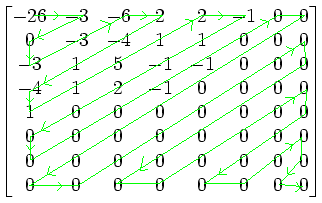
\includegraphics[width=2in]{figures/jpeg_zigzag.png}
    \end{center}
    \caption{The zigzag scanning used in JPEG intuitively maximizes the number of contiguous zeros encountered in the frequency matrix}
    \label{fig:zigzag}
\end{figure}
In this compression scheme, we take a much simpler approach by simply taking the output matrix of the 2D DCT type-2 and discarding the indices $k,l > m$ for $m \geq 1$ thereby constructing a low-rank approximation of the frequency matrix. This compression scheme is bound to have a higher data-loss rate as it simply ignores information that might be outside of this frame of the matrix. Relying on the assumption that most of the signal energy is concentrated in the lower spatial frequencies of the signal, this method should be a much better approximation than an arbitrary selection of $m\times m$ matrix elements.

One might be tempted to take this scheme and apply the transformation and rank reduction to the entire image in one two-dimensional DCT type-2. This method has two major flaws, the first being that our designed DCT only operates on square matrices while images can be any rectangular shape. We would have to either crop every image to a square or derive some type of padding scheme to extend the image bounds to a square. The second is that an unnecessary asymptotic complexity degree is used as our algorithm is $\mathcal{O}(n^2\log{n})$.

Instead, we can make our DCT a constant size and apply it to a disassembly of sub-matrices of the original signal. Our asymptotic runtime complexity is now $\mathcal{O}(n^2)$ and we have also somewhat solved the square image problem by reducing the proportions of the image that need to be padded or cropped. One question still remains regarding the size of these disassembled submatrices. We choose $8\times 8$ with no particular mathematical grounding, only noting that JPEG also chooses this size based on hardware constraints and empirical testing \cite{JPEG1992}.

The described process can be summarized in the following flow graphs with decompression being the regular construction of inverse operations:
\tikzstyle{startstop} = [rectangle, rounded corners, minimum width=2cm, minimum height=0.7cm,text centered, draw=black, fill=red!30]
\tikzstyle{filter} = [rectangle, minimum width=2cm, minimum height=0.7cm,text centered, draw=black, fill=green!50]
\tikzstyle{arrow} = [thick,->,>=stealth]


\begin{center}
    \begin{tikzpicture}[node distance=1cm]
        \node (image) [startstop, xshift=-2cm] {Image};
        \node (disassemble) [filter, right of=image, xshift=2cm] {Disassemble};
        \node (dct) [filter, below of=disassemble] {DCT II 2D};
        \node (reduce) [filter, left of=dct, xshift=-2cm] {Rank Reduce};
        \node (write) [startstop, below of=reduce, xshift=1cm] {Write Encoding};

        \node[draw] (compression) [above of=image, xshift=1cm] {Compression Pipeline};
        \node[draw] (decompression) [below of=compression, yshift=-4cm]{Decompression Pipeline};

        \node (read) [startstop, below of=decompression] {Read Encoding};
        \node (augment) [filter, below of=read, xshift=-2cm] {Augment Matrices};
        \node (idct) [filter, right of=augment, xshift=2.5cm] {DCT III 2D};
        \node (reassemble) [filter, below of=idct] {Reassemble};
        \node (im) [startstop, left of=reassemble, xshift=-1.5cm] {Image};

        \draw [arrow] (image) -- (disassemble);
        \draw [arrow] (disassemble) -- (dct);
        \draw [arrow] (dct) -- (reduce);
        \draw [arrow] (reduce) -- (write);
        \draw [arrow] (read) -- (augment);
        \draw [arrow] (augment) -- (idct);
        \draw [arrow] (idct) -- (reassemble);
        \draw [arrow] (reassemble) -- (im);
    \end{tikzpicture}
\end{center}

\subsection{Implementation and Results}
I implemented this using FFTW3 floating-point DCT transformations and a command-line program written in C. The source code can be found \href{https://github.com/henry-2025/math189-spectral-compression}{here}. The encoding, named JHPeg, achieves most of the functionality that I was hoping for with a few issues with rectangular-dimensioned images. As I anticipated, the use of floating-point math and type conversions makes this program run about 25 times slower than current JPEG encoders. However, the resulting files are comparable in size with a compression rate that retains somewhat acceptable image quality as shown in the following table:
\begin{center}
    \begin{tabular}{c|c c c}
        & JPEG & JHPeg & Uncompressed\\
        \hline
        Encoding Time & 0.12s & 3.10s & N/A\\
        File Size & 281K & 338K & 3.6M
    \end{tabular}
\end{center}
It is also helpful to observe the visual effects of low-rank approximation. Since the compression scheme is more unrefined than JPEG's we expect to see more inaccuracy in our image outputs. In \ref{fig:compression_outputs}, we observe these ``artifacts'' that are produced in the low-rank approximation images versus a state-of-the-art encoding..

\begin{figure}[h]
    \centering
    \begin{subfigure}[m]{0.5\textwidth}
        \centering
        
\includegraphics[width=\textwidth]{figures/lion_compare.jpg}
        \caption{A $960\times 960$ image with 75\% compression applied on the left(we have halved the ranks of the DCT matrices).}
        \label{fig:lion}
    \end{subfigure}
    \hfill
    \begin{subfigure}[b]{0.5\textwidth}
        \centering
        
\includegraphics[width=\textwidth]{figures/b_compare.jpg}
        \caption{A $256\times 256$ image with sharp edge features. Artifacts in the 75\% compression are more evident as seen in the compressed image on the left.}
        \label{fig:letter_b}
    \end{subfigure}
    \caption{Two different outputs of the compression algorithm that demonstrate its performance.}
    \label{fig:compression_outputs}
\end{figure}
\subsection{Conclusion}
Developing the compression scheme was enlightening because it tied together many of the insights from P\"uschel's work in a practical application that I already have a lot of appreciation for. He states that the task of deriving fast fourier transform algorithm from basic principles is greatly simplified through an algebraic approach. While I do believe this statement, designing an fft from the ground up was still too challenging a task to tackle in a single project. I think P\"uschel means that these understandings lead to systematic constructions of fast algorithms rather than their discovery by chance. This was certainly evident when I was able to reinterpret existing algorithms and apply them to new tasks.
\bibliographystyle{plain}
\bibliography{paper}
\end{document}